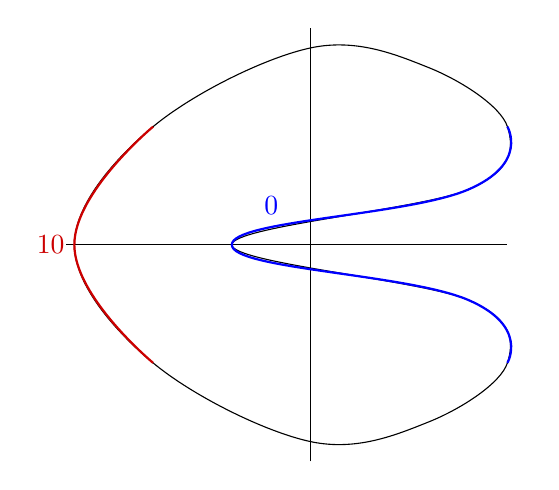
\begin{tikzpicture}
\draw[] (-3.1, 0) -- (2.5, 0);
\draw[] (0, -2.75) -- (0, 2.75);

\draw plot[smooth cycle, tension=0.6]
	coordinates {(-1,0) (2,0.7) (2.5, 1.5) (1.5, 2.25) (0, 2.5) (-2, 1.5) (-3, 0)
                              (-2, -1.5) (0, -2.5) (1.5, -2.25) (2.5, -1.5) (2, -0.7) };


% Colored regions
\draw[red!80!black, thick] plot[smooth, tension=0.8]  coordinates {(-2, 1.5) (-3, 0) (-2, -1.5)};
\draw[blue, thick] plot[smooth, tension=0.8]  coordinates {(2.5, -1.5) (2, -0.7) (-1,0) (2,0.7) (2.5, 1.5)};

\node[red!80!black, left] at (-3, 0) {$10$};
\node[blue] at (-0.5, 0.5) {0};

\end{tikzpicture}